%!TEX root=main.tex

A heurística 1, cujo o nome vem do facto de ter sido a primeira a ser implementada, tenta analisar as possibilidades de vitória para ambos os jogadores de uma forma relativamente ingénua. Para explicar como funciona observem-se os seguintes tabuleiros, onde os círculos a verde representam posições ocupadas pelo jogador 1, e a vermelhos as ocupadas pelo jogador 2.

\begin{table}[H]
\centering
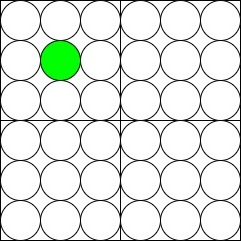
\includegraphics[height=4cm]{images/h1_block1.jpg}
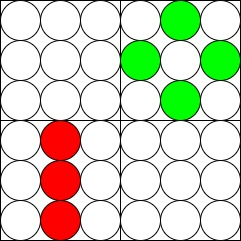
\includegraphics[height=4cm]{images/h1_block2.jpg}
\end{table}

Se atentarmos à segunda linha horizontal, em ambos os tabuleiros, podemos concluir rapidamente que o jogador 2 nunca poderá efetuar quatro em linha na segunda linha horizontal uma vez que esta se encontra bloqueada pelas peças do jogador 1. 

Podemos averiguar que temos 4 conjuntos de posições em cada um dos quadrantes que contêm a segunda linha horizontal. Quando um dos quadrantes fica com os 4 conjuntos ocupados por peças de um jogador deixa de ser possível ao jogador adversário usar essa linha para ganhar o jogo. As figuras seguintes ajudam a ilustrar esta situação no caso da segunda linha horizontal. 

\begin{table}[H]
\centering
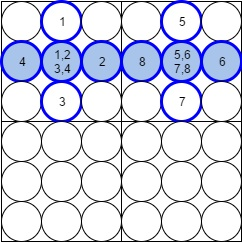
\includegraphics[height=4cm]{images/h1_pattern1.jpg}
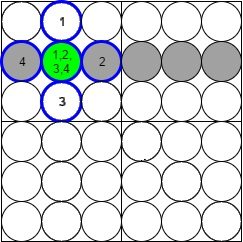
\includegraphics[height=4cm]{images/h1_block3.jpg}
\end{table}

A heurística 1 considera que o \emph{número de possibilidades} que um jogador tem para fazer 5 em linha na segunda linha horizontal é igual ao mínimo número de grupos livres (ainda não ocupados pelo adversário) entre os dois quadrantes que contêm a linha.
Este raciocínio é estendido para as outras linhas que podem ser usadas, sendo no caso das diagonais menores, considerados o mínimo de 3 quadrantes. As figuras seguintes ajudam a perceber o quais os grupos usados para cada linha em cada um dos quadrantes.

\begin{table}[H]
\centering
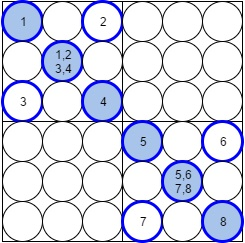
\includegraphics[height=4cm]{images/h1_pattern2.jpg}
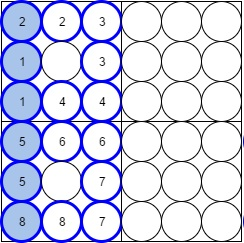
\includegraphics[height=4cm]{images/h1_pattern3.jpg}
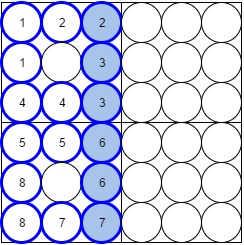
\includegraphics[height=4cm]{images/h1_pattern4.jpg}
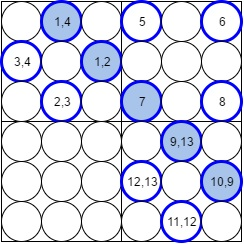
\includegraphics[height=4cm]{images/h1_pattern5.jpg}
\end{table}

A heurística inclui também uma variável \verb|bias| que permite dar mais peso às possibilidades dos jogador ou às possibilidades do jogador adversário. Assim é possível parametrizar a heurística de modo a que tenha um comportamento mais otimista, pessimista, defensivo ou ofensivo. A seguinte fórmula apresenta como é obtido um valor pela heurística, onde $Pm$ é o número de possibilidades para o próprio, $Po$ o número de possibilidades para o oponente e alfa a variável de \verb|bias|.

\begin{equation}
\alpha Pm-(1-\alpha)Po  \qquad\qquad\alpha\in[0,1] 
\end{equation}

Esta consideração é algo ingénua pois é possível que o adversário, fazendo uso das rotações, não permitir o uso de determinadas linhas enganando assim a heurística. Além disso se não é possível usar o minmax para evitar jogadas fatalistas no inicio do jogo, dado existirem demasiadas possibilidades a analisar, a heurística 1, isoladamente, não permite criar um adversário muito forte pois é muito passiva em relação ao estado do tabuleiro, não averiguando derrotas eminentes.

Foram também adicionados pesos aos diversos tipos de linhas. Assim, é possível ao algoritmo priorizar ou desprezar alguns tipos de linhas. Sem entrar em detalhe nos tipos de linhas considerados, intuitivamente estes pesos parecem ser importantes para desprezar as diagonais pequenas que não podem ser usadas em ataques de duas pontas e que ocupam 3 quadrantes. Foi realizada alguma experimentação com estes pesos mas não se chegou a uma solução ideal e não foram realizados testes similares aos apresentados nos anexos dado que já existiam demasiadas variáveis a testar. A adição destas nos testes ia aumentar o número de testes a realizar consideravelmente caso se testasse para todas as possíveis combinações dos \verb|biases|(pesos) na heurística 1 e 1.2.

